\chapter{Human Robot Interaction}

During this chapter, we will be talking about the interaction between humans and robots, and how to design interfaces that allow for effective communication and collaboration between the two. However, before we dive into it, it is important to understand what a \emph{robot} is. A robot is a multi-purpose machine that can be programmed to perform a variety of tasks emulating living beings. They are therefore mobile and autonomous. The three esential aspects of a robot are:
\begin{itemize}
    \item \ul{Sensing}: The ability to perceive the environment through sensors, such as cameras, microphones, and touch sensors.
    \item \ul{Thinking}: The ability to process information and make decisions based on the data received from the sensors.
    \item \ul{Acting}: The ability to perform actions based on the decisions made by the robot, such as moving, manipulating objects, or communicating with humans.
\end{itemize}

Since robots are becoming more common in our daily lives, it is crucial to correctly understand the Human Robot Interaction (HRI), specially because of the \emph{social} aspect of it. Even though robots may have a correct physical interaction because of their sensors and actuators, they may fail to interact with humans in a way that is socially acceptable or effective. HRI is a multidisciplinary field therefore focuses on developping robots that can interact with humans in a natural and intuitive way.

\section{Classifications in HRI}

When working in HRI, plenty of different  classifications should be taken into account. However, the most important ones are:
\begin{itemize}
    \item Robot classification depending on their interaction capabilities.
    \item Human classification depending on their role in the interaction.
    \item Interaction classification depending on the type of interaction between humans and robots.
\end{itemize}

Depending on their interaction capabilities, we can classify robots into different categories:
\begin{itemize}
    \item \ul{Bounded Autonomy}: Robots with limited autonomy that operate within predefined constraints.
    \item \ul{Teleoperation}: Robots controlled remotely by a human operator.
    \item \ul{Supervised Autonomy}: Robots that operate autonomously but under human supervision.
    \item \ul{Adaptive Autonomy}: Robots that can adapt their behavior based on the environment and user needs.
    \item \ul{Virtual Symbiosis}: Robots that collaborate with humans in a way that enhances both parties' capabilities. The robot is a co-worker.
\end{itemize}
% // TODO: Add descriptions for each category of robots.

Depending on the role of humans in the interaction, we can classify them into different categories:
\begin{itemize}
    \item \ul{Supervisor}: The human is responsible for overseeing the robot's actions and ensuring that it operates safely and effectively.
    \item \ul{Operator}: The human is responsible for controlling the robot's actions, either directly or through a user interface.
    \item \ul{Mechanic}: The human is responsible for maintaining and repairing the robot, ensuring that it remains in good working condition.
    \item \ul{Peer}: The human is a collaborator with the robot, working together to achieve a common goal.
    \item \ul{Bystander}: The human avoids interaction with the robot, either because they are not interested or because they are afraid of it.
\end{itemize}

Depending on the type of interaction between humans and robots, we can classify them into different categories:
\begin{itemize}
    \item \ul{Coexistence}: The human and the robot share the same environment at the same time, but they do not interact with each other.
    \item \ul{Cooperation}: The human and the robot share the same environment at the same time, and they interact with each other to achieve a common goal.
    \item \ul{Collaboration}: The human and the robot share the same environment at the same time, and they interact with each other to achieve a common goal, depending on each other to achieve it.
\end{itemize}

\section{Development of a Robot}

When developing a robot, there are several different aspects that should be taken into account. In order to design it, a modular approach should be taken, and the \emph{three main components of the robot} are considered from the  sense-think-act approach:
\begin{itemize}
    \item \ul{Perception} (Hardware and Software):
    
    Both self monitoring and environment perception are crucial for a robot to interact effectively with humans.
    \begin{itemize}
        \item \emph{Self monitoring}: The robot should be able to monitor its own state, such as its battery level, motor status, and sensor readings.
        \item \emph{Environment perception}: The robot should be able to perceive the environment through sensors, such as cameras, microphones, and touch sensors.
    \end{itemize}
    \item \ul{Cognition} (Software):
    
    The robot should have a cognitive architecture that allows it to process information and make decisions based on the data received from the sensors. It runs on operating systems, such as ROS (Robot Operating System), that provide a framework for developing and deploying robot software.

    Their skills are usually preprogrammed, but they can also learn from experience and adapt to new situations (machine learning). Most of their learning capabilities are offline, but active research is being done in online learning, which allows robots to learn and adapt in real-time.
    \item \ul{Action} (Hardware and Software):
    
    In order to perform actions, the robot should have actuators, such as motors and grippers, that allow it to move and manipulate objects.
\end{itemize}

Once the three main components of the robot are defined, the design of the interaction can be done. Two different approaches are:
\begin{itemize}
    \item \ul{Inside-out approach}: The design starts by building the technology, and the interaction is designed around it. It is later tested by social scientists, who evaluate the interaction and provide feedback to the engineers.
    \item \ul{Outside-in approach}: The design starts by understanding the social context and the needs of the users, and then the technology is developed to meet those needs. 
\end{itemize}

When designing the robot, there are different aspects that should be considered regaring the interaction with humans. Some of the most important ones are:
\begin{itemize}
    \item \ul{Morphology}: The physical design of the robot, which can affect how humans perceive and interact with it. It should take into account several factors:
    \begin{itemize}
        \item The form and their function should be consistent.
        \item Android robots (those that physically resemble humans) should be designed with care, as they may be antropomorphic. In addition, the \emph{uncanny valley} phenomenon should be taken into account (Figure~\ref{fig:uncanny-valley}), which describes the discomfort that humans may feel when interacting with robots that are very close to human appearance, but not quite there.
        \begin{figure}
            \centering
            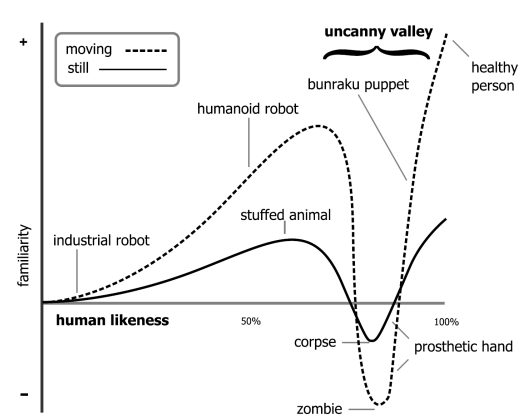
\includegraphics[width=0.7\textwidth]{img/UncannyValley.png}
            \caption{The uncanny valley phenomenon.}
            \label{fig:uncanny-valley}
        \end{figure}
        \item Antropomorphic robots (those that are attributed with human traits or emotions) should be designed with care, as they may create unrealistic expectations about their capabilities. There are several questionnaires that can be used to evaluate the antropomorphism of a robot, such as the Godspeed questionnaire.
        
        It should be noted that android are more tend to be antropomorphic, but these are not the same thing. For example, a robot that looks like a dog may be antropomorphic, but it is not an android. In addition, computers can also be antropomorphized when humans shout at them, but they are not robots.
    \end{itemize}
    \item \ul{Affordances}: The design of the robot should provide clear affordances that indicate how it can be interacted with. For example, a robot with a handle may indicate that it can be picked up, while a robot with a screen may indicate that it can be interacted with through touch.
    \item \ul{Underpromise and overdeliver}: Expectations should be defined clearly, and the robot should be designed to exceed those expectations.
    \item \ul{Interaction expands functionality}: On open-ended design should be taken, allowing for the interaction to expand the functionality of the robot beyond its initial design. For example, a robot designed for cleaning may also be able to provide companionship and social interaction.
\end{itemize}